\customHeader{1}{\neuralNetwork{}s}
\label{02_neural_networks}

In this section, we present the fundamental concepts necessary for understanding \neuralNetwork{}s, drawing on the Open Access material from \mytextcite{deep_learning_introduction} and \mytextcite{wolfram_llm}.

\todo{Quickly Explain:} 
\begin{itemize}
    \item \todo{neurons}
    \item \todo{activation function}
    \item \todo{Loss}
    \item \todo{training: e.g. with gradient descent}
    \item \todo{back propagation}
    \item \todo{optimizers}
    \item \todo{feed-forward neural networks}

    %\item \todo{MLP}
    %\item \todo{Logistic Regression}
    \item \todo{RNNs (LSTM, GRU)}
    \item \todo{Attention}
    \item \todo{Transformers}
    \item \todo{BERT}
\end{itemize}

\customHeader{2}{Motivating Example}
\label{02_nn_motivating_example}

To motivate why we use neural networks, imagine we want to know how the temperature and humidity of a location corresponds to the temperature felt by living organisms like humans. That is, given these two values in several locations, we would like to predict the apparent temperature or heat index at each location. We could consider a simplified version of the model presented in  \cite{heat_index}, and have the following equation for the Heat Index ($HI$):

\begin{align*}
    HI &= w_{Temp} T + w_{Hum} H + c
\end{align*}


The main idea behind this model is that the heat index, our \emph{target}, can be calculated as a weighted sum of the temperature $T$ and the humidity $H$. The influence of $T$ on the $HI$ is given by $w_{Temp}$ and that of $H$ by $w_{Hum}$, and we correct by a constant value $c$. 

For this model, $H$ and $T$ are called the \emph{features} of a location, and they characterize the location, that is, all locations with the same features will produce the same output. Here, $w_{Temp}, w_{Hum}$ are called \emph{weighs} or \emph{parameters}, and they determine how important the features are for the model, for example, if $w_{Hum}$ were zero, the $HI$ would only depend on $T$. Also, $c$ is called the \emph{bias} or \emph{offset}, and it is the value of the output when the features are zero.
Finally, the weighted sum at right-hand side of the equation, $w_{Temp} T + w_{Hum} H + c$, is known as the \emph{output} or \emph{prediction} of the model.

In reality, the weights and bias of this model are known:
\begin{align*}
    w_{Temp} & = 1.1\\
    w_{Hum} &= 0.047 \\
    c &= -10.3
\end{align*}

However, this simplification is limited. As it turns out, we can obtain better results by adding one more calculation step. Consider the squaring function $f(u) = u^2$, then, our model becomes:


\begin{align*}
    HI &= f(w_{Temp} T + w_{Hum} H + c)
\end{align*}

For this improved model, $f$ is called and \emph{activation function}, and the prediction or output is the result of applying $f$ to the weighted sum. By adding this additional computation, we are able to better replicate how living organism react to big changes in temperature and humidity. This kind of model allows us to use numerical features, to obtain a prediction for a quantity we care about.


\customHeader{2}{Neurons}
\label{02_nn_neurons}

As we work with more and more complicated phenomena, we cannot write the new models explicitly with few features and parameters, and thus we need to generalize this idea. 
In Machine Learning, \emph{neurons} are a generalization of the kind of model presented above. 




\begin{figure}[ht]
    \centering
    \subfigure[Neuron overview]{
    \begin{tikzpicture}[scale=0.7, every node/.style={transform shape}]
        % Add the "Hello" text to the left
        \node[anchor=east] at (-3, 0) {Input};
        
        % Draw the neuron circle with a node name
        \node[draw, thick, circle, minimum size=1.5cm, fill=mylightblue] (neuron) at (0, 0) {};
        
        % Draw the input nodes with labels x_i
        \foreach \x/\xval in {1/{$x_1$}, 2/{$x_2$}, 3/{$x_3$}} {
            \node[draw, circle, minimum size=0.7cm] (input\x) at (-2, 2.8-\x*1.4) {};
            \draw[->] (input\x) -- node[above] {} (neuron);
        }
        
        % Draw the output arrow
        \draw[->] (neuron) -- (2, 0) node[right] {Output};
    \end{tikzpicture}
    }
    \hfill
    \subfigure[Neuron with weights]{
    \begin{tikzpicture}[scale=0.7, every node/.style={transform shape}]
        % Add the "Hello" text to the left
        \node[anchor=east] at (-3, 0) {Input};
        
        % Draw the neuron circle with a node name
        \node[draw, thick, circle, minimum size=1.5cm, fill=mylightblue] (neuron) at (0, 0) {$f$};
        
        % Draw the input nodes with labels x_i
        \foreach \x/\xval in {1/{$x_1$}, 2/{$x_2$}, 3/{$x_3$}} {
            \node[draw, circle, minimum size=0.7cm] (input\x) at (-2, 2.8-\x*1.4) {\xval};
            \draw[->] (input\x) -- node[above] {$w_\x$} (neuron);
        }
        
        % Draw the output arrow
        \draw[->] (neuron) -- (2, 0) node[right] {$z$ Output};
    \end{tikzpicture}
    }
    \caption{
    Basic Neuron
    }
    \label{fig:02_neuron}
\end{figure}


Consider a model where the  inputs consist of $n$ features, $(x_1, x_2,\ldots,x_n)$; the diagram in Figure \ref{fig:02_neuron} is used to represent the following equation:

\begin{align*}
    z &= f(w_1 x_1 + w_2 x_2 + \ldots + w_d x_d + b)
\end{align*}

where $w_1, w_2,\ldots,w_n$ are the weights, $b$ is the bias, $f$ is the activation function, and $z$ is the prediction.

One of the main insights in \gls{ml} is that one does not need to manually define the parameters $(w_1, w_2,\ldots,w_n,b)$ for this kind of model, instead, given a lot of data containing features and observed values of the target, one can find the optimal values for the parameters, such that the predictions of the model are as close as possible to the observed target values. After this, one can use the model for new data. The process of finding the optimal parameters is called \emph{training}.

In order to find the optimal parameters, we first need to decide how to produce our final predictions, how to measure how well the model is performing, and how to update the parameters.


\customHeader{2}{Activation functions}
\label{02_nn_activation_functions}

How our final predictions are calculated depends on the kind of problem we are addressing. For different problems, different activation functions are available, and in some cases, they can be combined. For example, for \emph{regression}, that is, when we want to calculate some index, like in the example in \headerName{} \ref{02_nn_motivating_example}, we are dealing with values that may be very small or very large. For \emph{classification}, as explained in \headerName{} \ref{02_text_classification}, we are dealing with probabilities of belonging to different categories.

Some of the most common activation functions are listed in Table \ref{tab:02_nn_common_activation_functions}: 

\begin{table}%[]
    \centering
    \begin{tabular}{p{4cm}|p{8cm}}
        \textbf{Activation Function} &  \textbf{Description} \\ \hline
        Identity &  No modification to the weighted sum\\
        \gls{relu} & Eliminates negative values. Better for optimization \\
        \gls{sigmoid} & Outputs a single probability \\
        \gls{softmax} & Generalization of \gls{sigmoid} for multiple categories. Outputs a list of probabilities. \\
        \gls{tanh} & Reduces the influence of huge and minuscule values. Better for optimization \\
    \end{tabular}
    \caption{Common activation functions}
    \label{tab:02_nn_common_activation_functions}
\end{table}


\begin{figure}[ht]
    \centering
    \subfigure[Identity]{
        \begin{adjustbox}{max height=0.07\textheight}
            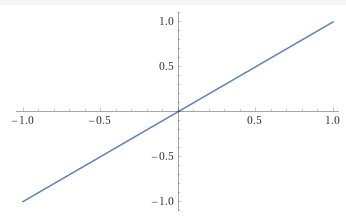
\includegraphics[width=0.45\textwidth]{Figures/02/Activation_functions/02_Identity.png}
        \end{adjustbox}
        
        %\label{fig:image1}
    }
    \hfill
    \subfigure[ReLU]{
        \begin{adjustbox}{max height=0.07\textheight}
            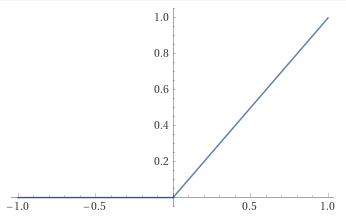
\includegraphics[width=0.45\textwidth]{Figures/02/Activation_functions/02_Relu.png}
        \end{adjustbox}
        
        %\label{fig:image2}
    }
    \hfill
    \subfigure[Sigmoid]{
        \begin{adjustbox}{max height=0.07\textheight}
            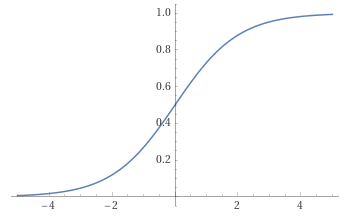
\includegraphics[width=0.45\textwidth]{Figures/02/Activation_functions/02_sigmoid.png}
        \end{adjustbox}
        
        %\label{fig:image1}
    }
    \hfill
    \subfigure[Tanh]{
        \begin{adjustbox}{max height=0.07\textheight}
            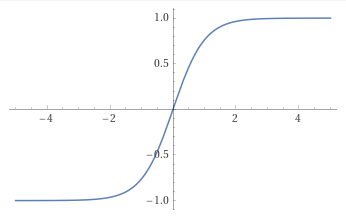
\includegraphics[width=0.45\textwidth]{Figures/02/Activation_functions/02_tanh.png}
        \end{adjustbox}
        
        %\label{fig:image2}
    }
    \caption{Common activation functions}
    \label{fig:02_nn_common_activation_functions}
\end{figure}





\customHeader{2}{Loss Functions}
\label{02_nn_loss_functions}

Loss functions are how we measure how far our neuron's predictions are from the real target values. The objective of training is to find the parameters that minimize our loss. Feeding the input into the neuron in order to calculate the loss is called the \emph{forward pass}.
For different problems, different loss functions are available. For regression problems, it is common to use the squared error, which measures the Euclidean distance between the prediction and the real value:

\begin{equation}
    loss_{SE}(x,w,b) =  \dfrac{1}{2} (z_{pred}(x,w,b)-z_{real})^2
\end{equation}

where $z_{pred} = f(xw+b)$.
%Note that the loss depends on the weights ($w = (w_1, w_2, \ldots, w_n)$) and the bias, since the features and real target value are given, and calculating the prediction needs the weights and the bias.

For classification problems, it is common to use the \emph{cross-entropy}. Though deducing it is outside the scope of this project, the important thing to remember is that minimizing cross entropy is equivalent to maximizing the confidence with which our neuron assigns categories.

If, for features $x = x_1, x_2, \ldots, x_n$ we predict probabilities $p_1, p_2, \ldots, p_k$ for categories $c_1, c_2, \ldots, c_k$, and encoding the real categories as $(q_1, q_2, \ldots, q_k)$ where $q_j =1 $ if $x$ belongs to category $j$ and $q_j = 0$ otherwise, then, the cross entropy is calculated as:

\begin{equation}
    loss_{CE}(x,w,b) =  - \sum_{j} q_{j}(x) \log{(p_{j}(x,w,b))}
\end{equation}

In the case of an \emph{unbalanced} dataset for classification, that is, when the categories are not uniformly distributed, we may use a variant of $CE$ called \emph{weighted cross-entropy}, which scales up the cross-entropy for the less represented categories, and vice versa. If each category $j$ is assigned a factor of $r_j$, then:

\begin{equation}
    loss_{WCE}(x,w,b) =  - \sum_{j} r_j q_{j}(x) \log{(p_{j}(x,w,b))}
\end{equation}

\customHeader{2}{Backpropagation}
\label{02_nn_loss_back_propagation}

Once the loss informs us of how well a neuron is performing, we would like to change its parameters in order to minimize the loss. Updating the weights in order to minimize the loss is called \emph{backpropagation}.
One optimization technique for this is called \emph{gradient descent}.  For simplicity of explanation, consider that there was only one parameter or weight for calculating the loss (Figure \ref{fig:02_nn_gradient_descent}). The important observation is to see that, when going against the slope of the curve, one approaches the minimum. This slope is called the derivative or \emph{gradient} of the loss function. Eventually, after several incremental steps which takes us to a new weight, we end up finding the optimal weight that minimizes the loss.

\begin{figure}
    \centering
    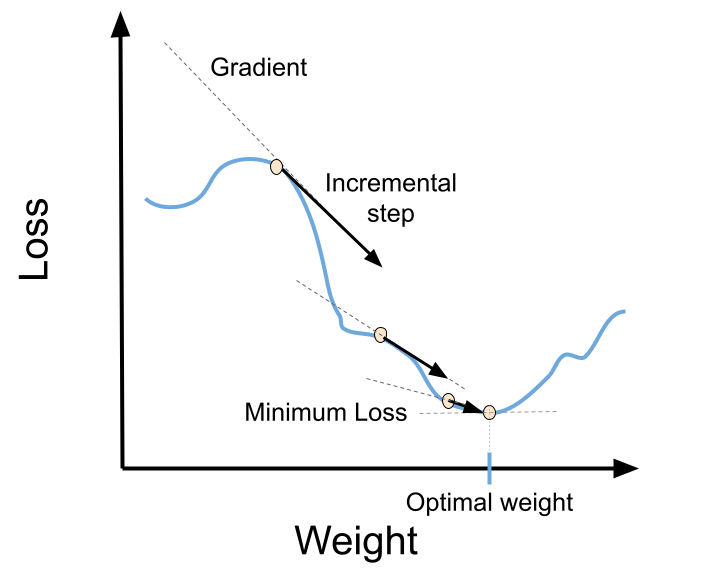
\includegraphics[width=0.5\textwidth]{Figures/02/02_gradient_descent.png}
    \caption{Gradient descent}
    \label{fig:02_nn_gradient_descent}
\end{figure}

Once we know in which direction to go, we may also want to control how much into that direction to go. For this, we introduce the \emph{learning rate} $\gamma$, which controls the influence of the gradient in updating the weights. That is, our weight updating process looks like:

\begin{align}
    w_{new} = w_{old} - \gamma \nabla Loss(x, w_{old})  \label{eq:02_nn_gradient_descent}
\end{align}

% gradient descent
% learning rate
% loss optimization

\customHeader{2}{Training}
\label{02_nn_training}

Until now, we have only considered passing on a single feature vector. However, for training, we need more than one data point, that is, we need a dataset of features and observed target values $(x,z_{real})$. If our dataset $D$ has $N$ entries, our objective is to minimize the \emph{average} loss over the dataset:

\begin{equation}
    Loss(w,b) =  \dfrac{1}{N} \sum_{x\in D} loss(x,w,b)
\end{equation}

The whole cycle of performing the forward pass, calculating the loss, and updating the parameters is called an \emph{epoch} (Figure \ref{fig:02_nn_neuron_training}). 

\begin{figure}
    \centering
    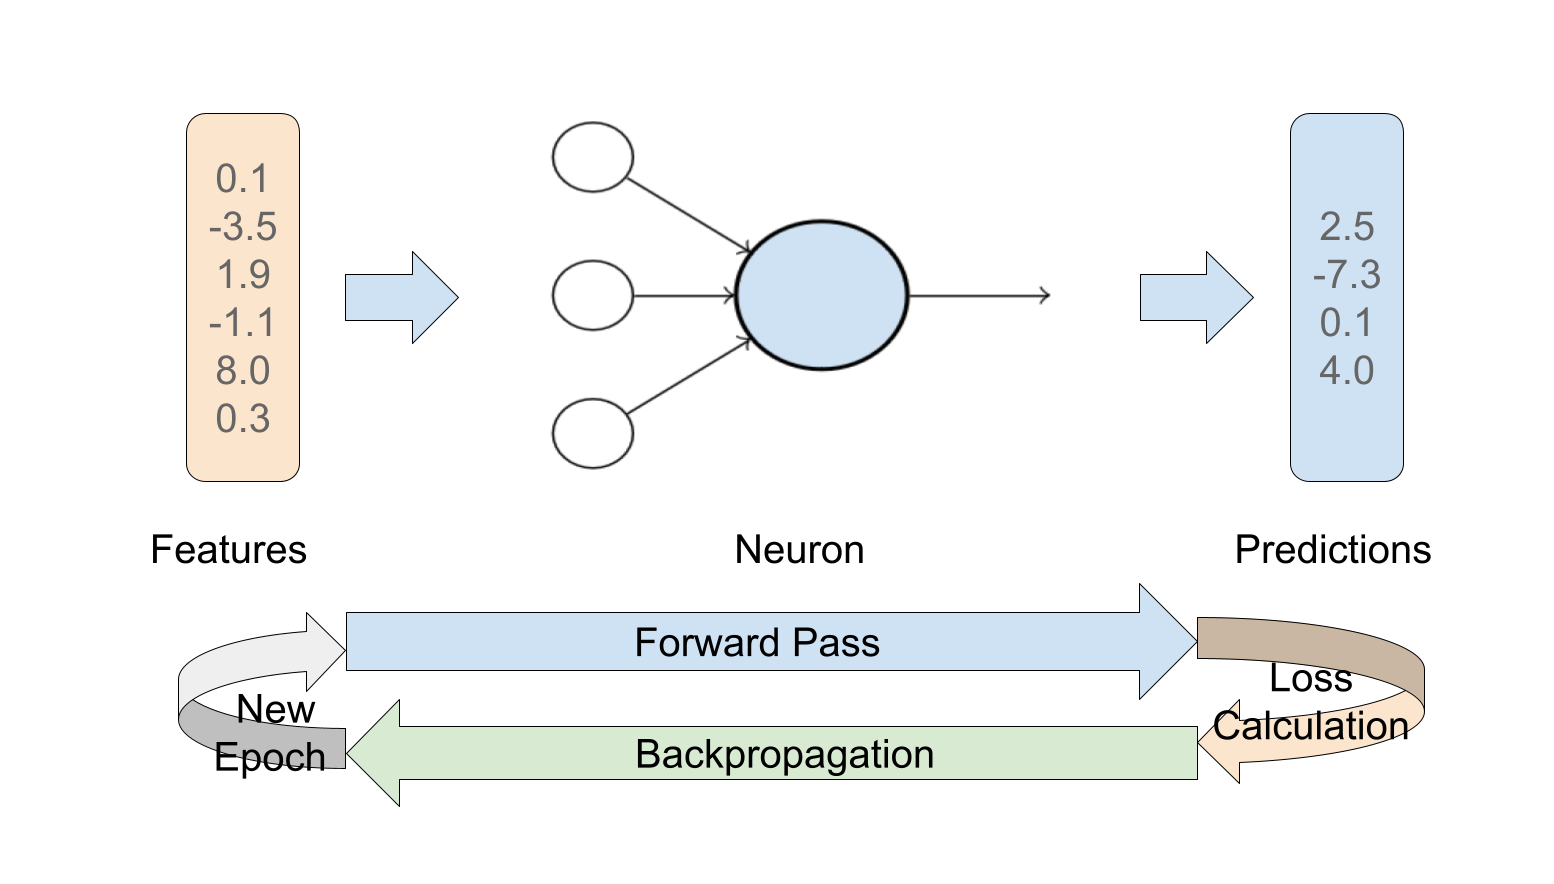
\includegraphics[width=0.5\textwidth]{Figures/02/02_neuron_training.png}
    \caption{Training a Neuron}
    \label{fig:02_nn_neuron_training}
\end{figure}

Usually,  our hardware will not have enough memory to do the forward pass for the complete dataset. To avoid this issue, it is common to divide the dataset in \emph{batches}, and then do the forward pass and loss calculation on each batch until the whole dataset is processed. Afterwards, the losses for each batch are aggregated to obtain the final loss, and the backpropagation is performed.

Usually, a single epoch is not enough to obtain decent results. Thus, it is common to train a neuron for several epochs. After each epoch, we usually obtain a smaller loss (Figure \ref{fig:02_nn_loss_evolution}).

\begin{figure}
    \centering
    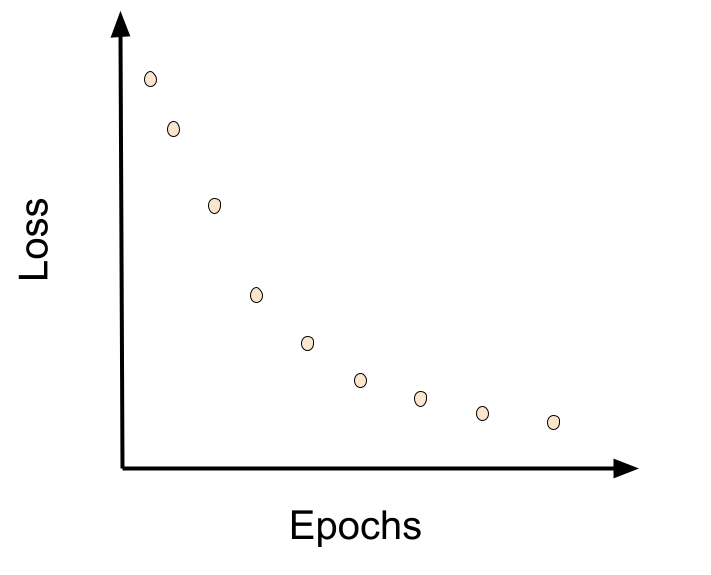
\includegraphics[width=0.5\textwidth]{Figures/02/02_loss_evolution.png}
    \caption{Evolution of loss during training}
    \label{fig:02_nn_loss_evolution}
\end{figure}

% batches
% epochs

\customHeader{2}{Overfitting }
\label{02_nn_overfitting}

As we minimize our loss, a problem arises. Sometimes the neuron will have excellent predictions for the data we showed it during training, yet  fail when seeing completely new data, thus rendering it useless for applications. This phenomenon is called \emph{overfitting}. 

One common way to avoid overfitting is to \emph{split} a dataset into three components:

\begin{enumerate}
    \item A \emph{training} split, which is a portion of the dataset used for the actual training, that is, the forward pass, loss calculation, and crucially, backpropagation.
    \item A \emph{development} split, which is a portion of the dataset used for tracking overfitting. For the development split, we calculate the forward pass and loss, and sometimes other metrics, but there is no backpropagation. After we notice when overfitting starts, we can adjust our setup for the optimal number of epochs.
    \item A \emph{test} split, which is a portion of the dataset used for evaluating performance of the final setup chosen for training, since it had no influence in selecting such setup.
\end{enumerate}

While tracking the evolution of the loss across the training and development splits, one notices that after some epochs, while the loss on the training split keeps decreasing, the loss on the development split increases. This signals the moment in which overfitting starts (Figure \ref{fig:02_nn_split_loss_evolution}).

\begin{figure}
    \centering
    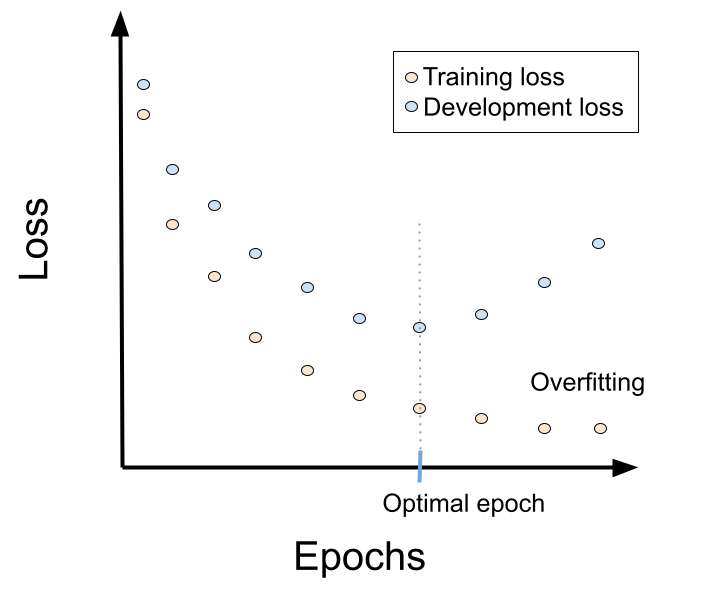
\includegraphics[width=0.5\textwidth]{Figures/02/02_split_loss_evolution.png}
    \caption{Evolution of loss on the training and development splits}
    \label{fig:02_nn_split_loss_evolution}
\end{figure}


% splits.
% plot for optimal epoch

\customHeader{2}{Optimizers }
\label{02_nn_optimizers}

% optimizers
We may generalize gradient descent (Equation \ref{eq:02_nn_gradient_descent}), by noticing that we only need to calculate some way to update our weights:

\begin{equation}
    w_{new} = w_{old} - \texttt{Update}(x, w_{old})
\end{equation}

Different optimization methods calculate the \texttt{Update} in different ways. Software implementations of these optimization methods are called \emph{optimizers}. Some common methods are listed in Table \ref{tab:02_nn_common_optimizers}, listed by increasing performance.

\begin{table}%[]
    \centering
    \resizebox{\textwidth}{!}{
    \begin{tabular}{p{5cm}|p{8cm}}
        \textbf{Optimization method} &  \textbf{Description} \\ \hline
        Gradient Descent &  Classical Gradient Descent\\
        Stochastic Gradient Descent (SGD) & Estimates the gradient by only using randomly subset of the data \\
        SGD with Momentum & Uses the estimated gradient and the previous value of \texttt{Update}\\
        Averaged SGD &  Takes into account several past values of \texttt{Update} and averages them while giving less importance to older values \\
        Adaptive Gradient (AdaGrad) & A version of SGD where each weight is updated individually, instead of all at the same time. It calculates \texttt{Update} by averaging and normalizing over the history of updates \\
        Adam & AdaGrad + Momentum \\
        AdamW & Extension of Adam, controling for the magnitude of each weight \\
    \end{tabular}
    }
    \caption{Common optimization methods for backpropagation}
    \label{tab:02_nn_common_optimizers}
\end{table}


\customHeader{2}{Feed-Forward \neuralNetwork{}s}
\label{02_nn_ffnn}

As we have seen, an individual neuron may take several inputs to give an output. 
One of the biggest insights of \gls{ml} was to notice that one obtain systems with a lot of predictive power by connect neurons, that is, by giving the output of one neuron as input for another one. By stacking \emph{layers} of neurons in a network pattern, one obtains a \gls{ffnn} (Figure \ref{fig:02_nn_ffnn}). 
\footnote{All \neuralNetwork{} diagrams were made with the $NN-SVG$ drawing tool by \mytextcite{drawing_nns}}

\begin{figure}
    \centering
    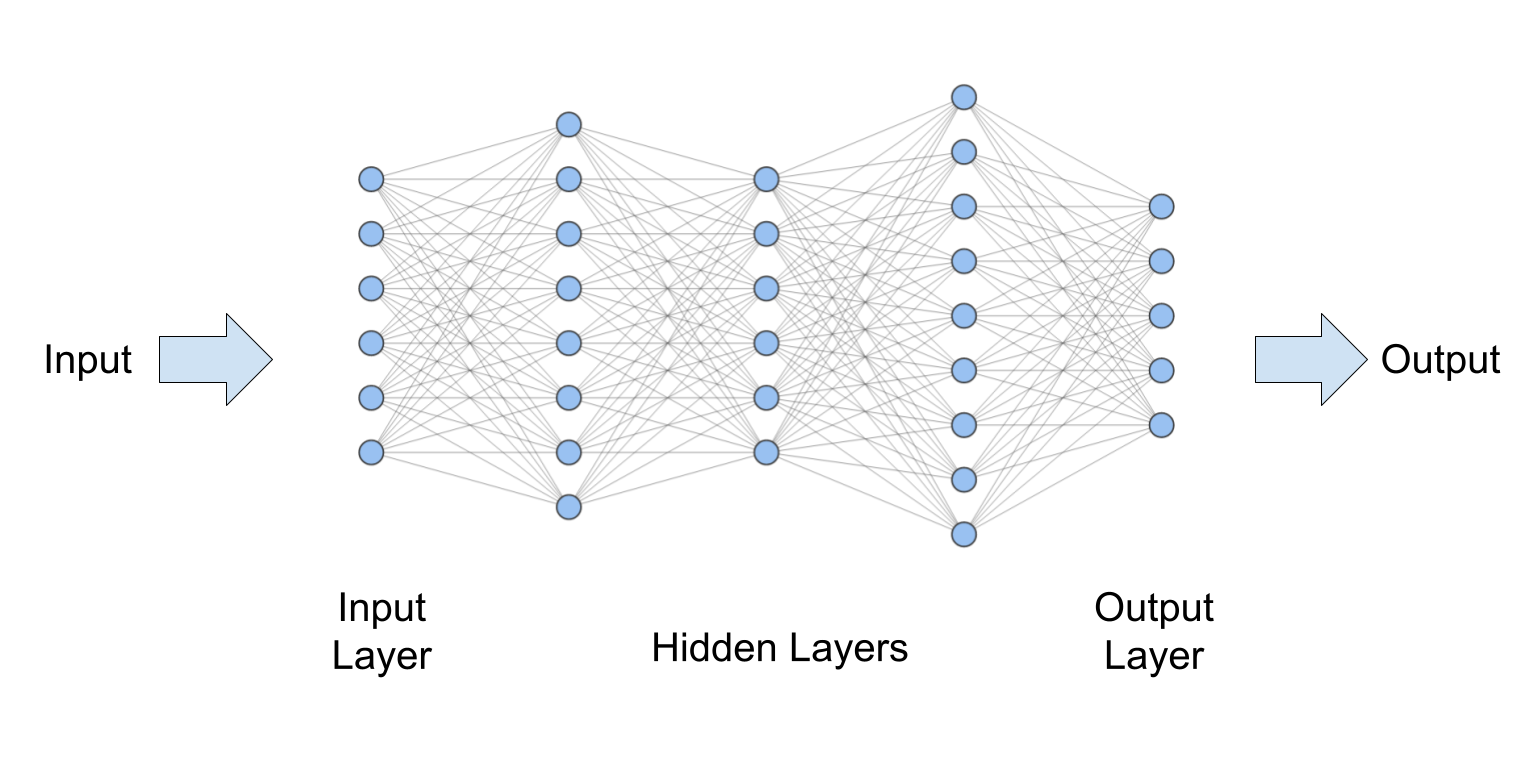
\includegraphics[width=0.5\textwidth]{Figures/02/02_FFNN.png}
    \caption{A Feed-Forward \neuralNetwork{}}
    \label{fig:02_nn_ffnn}
\end{figure}

As we feed the input features to the \gls{ffnn} through the \emph{input layer}, the data passes through the intermediate layers up to the \emph{output layer}. As the \gls{ffnn} is trained, each intermediate layer will produce new features to feed into the next layers. In this way, the \gls{ffnn} \emph{learns} new representations of the data. These intermediate, or \emph{hidden} features exploit patterns in the previous features to influence the final output of the \neuralNetwork{}. A \neuralNetwork{} with only one hidden layer is called \emph{shallow}, while one with multiple hidden layers is called \emph{deep}.

For classification tasks, it is common to use a \gls{softmax} activation function for the output layer, as it produces an array of probabilities of belonging to each category. This kind of layer is called a \emph{\gls{softmax} layer} or a \emph{classification layer}. The inputs to a \gls{softmax} layer are called \emph{logits} (Figure \ref{fig:02_nn_nns_for_classification}).

\begin{figure}
    \centering
    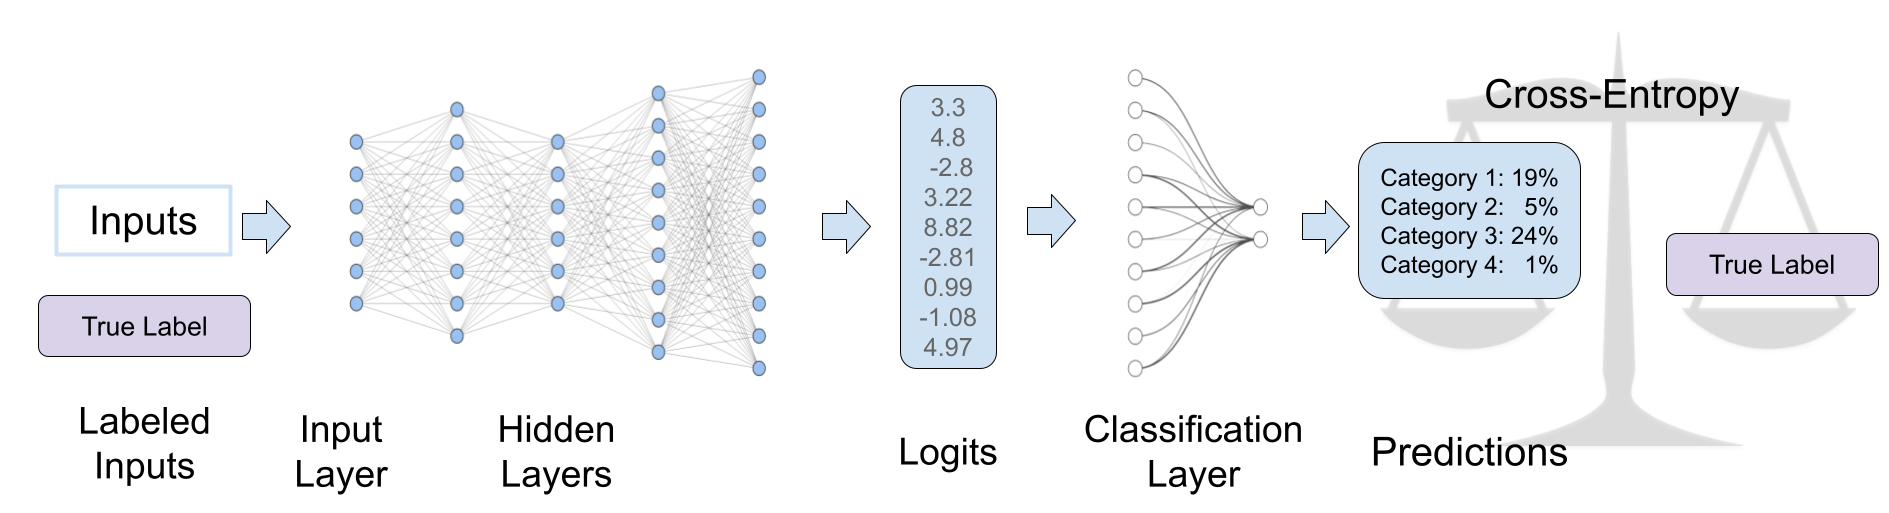
\includegraphics[width=\textwidth]{Figures/02/02_nns_for_classification.png}
    \caption{\neuralNetwork{}s for Classification Tasks}
    \label{fig:02_nn_nns_for_classification}
\end{figure}


% FF NN
% deep vs shallow
% softmax layers
% diagram with the full training cycle

\customHeader{2}{Hyperparameters}
\label{02_nn_hyperparameters}

A \neuralNetwork{} is trained to find the optimal parameters or weights to minimize its loss. However, there are several decisions left to the ones implementing the neural network.

Some decisions concern the \emph{architecture} of the \neuralNetwork{}, such as:

\begin{itemize}
    \item Number of layers
    \item Number of Neurons per layer
    \item Activation functions for each layer
    \item Dimension of output features
    \item Loss function
    \item Optimizer
\end{itemize}

Other decisions concern numerical values that influence the training algorithm, such as, 

\begin{itemize}
    \item Number of epochs
    \item Learning rate
    \item Batch size
    \item Sizes for the dataset splits
\end{itemize}

All these are known as \emph{hyperparameters}. Unfortunately, there is no one-size-fits-all answer to the question of which hyperparameters to use because the optimal hyperparameters can vary depending on the specific dataset, model architecture, and task at hand. The search space for hyperparameters can be vast, and finding the best combination can be computationally expensive and time-consuming. As a result, the choice of hyperparameters is often determined through trial and error, experimentation, and a combination of domain knowledge and experience.

%% Hyperparameters
% learning rate
% epochs
% batch size
% training, dev, and test split size


%% architecture
% dimension of input features
% activation functions
% number of layers
% neurons per layer

\customHeader{2}{\neuralNetwork{}s for NLP tasks}
\label{02_nn_nlp_tasks}

In order to use \neuralNetwork{}s for NLP tasks, one needs to have numerical features for textual data to feed to the network.
A big breakthrough in \gls{nlp} came when researchers realized that, instead of manually designing algorithms to produce features, one can train \neuralNetwork{}s to produce the features to be given to other \neuralNetwork{}s. The following section is dedicated to explaining this process.



%\clearpage